\scanpage{88}
\mspage{20}
points. D'après la théorie générale des groupes fondamentaux mixtes et de leurs relations avec les groupes fondamentaux à signature, on trouve donc un isomorphisme (extérieur pour le moment) canonique
\[
\tag{93}
\begin{aligned}
\Pi_1(X_n^*,\underset{\substack{\Vert\\0}}{\underline{P_{n+}}})_{\unsure{*|D}}
&\overset\sim\longrightarrow
\Pi_1(\underset{X_0\setminus\{0\}}{\underline{X_0^{\inserted{*}}}}\deleted{\unsure{,\{0\}}},2\{1\}+n\{\infty\};\underset{\exp 2i\pi/6}{\underline{P_{0+}}})\\
&\simeq\Pi_1(\underset{\mathbb P^1(\mathbb C)}{\underline{X_0}},\infty\{0\}+2\{1\}+n\{\infty\};P_{0+}).
\end{aligned}
\]
Pour trouver un isomorphisme pas extérieur, il faut changer le point base $P_{n+}=0$ en un autre, qui s'en aille dans
$\deleted{\unsure{X_0^*\setminus\{1,\infty\}}}\quad X_0^*\setminus\{1,\infty\}=X_0\setminus\{0,1,\infty\}=U_{03}$.

\figure{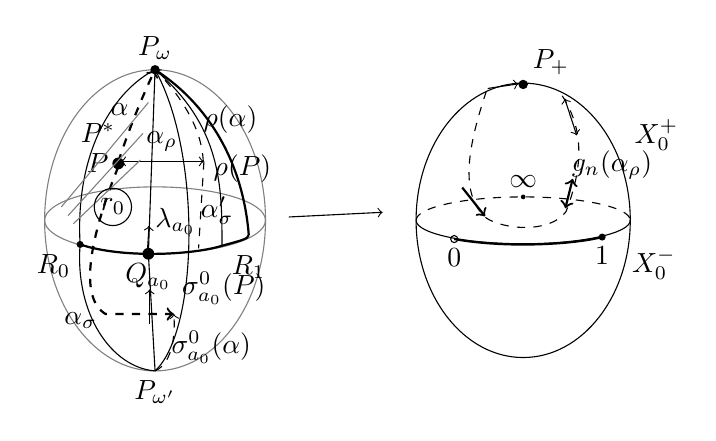
\begin{tikzpicture}[x=1cm,y=1cm,scale=.85]
\begin{scope}
\draw[gray] (0,0) ellipse (1.65 and 2.25);
\draw[gray] (-1.65,0) arc[start angle=180,end angle=360,x radius=1.65,y radius=.5];
\draw[gray] (-1.65,0) arc[start angle=180,end angle=0,x radius=1.65,y radius=.5];
\draw (-1.12,-.36) .. controls (-1.2,1.05) and (-.6,1.95) .. (0,2.25)
 .. controls (1,1.4) and (1.0,.5) .. (1,-.38);
\draw (0,2.25) .. controls (.7,1) and (.65,-1.65) .. (0,-2.25);
\draw (-1.12,-.36) .. controls (-1.2,-1.4) and (-.65,-2.2) .. (0,-2.25);
\draw[thick] (-1.12,-.36) .. controls (-.5,-.57) and (.55,-.52) .. (1,-.38)
 .. controls (1.25,-.31) and (1.4,-.28) .. (1.4,-.22);
\draw[thick] (1.4,-.22) .. controls (1.32,.8) and (.85,1.7) .. (0,2.25);
\draw (0,2.25) -- (-.1,-.5) -- (0,-2.25);
\fill (0,2.25) circle (2pt); \node[above] at (0,2.25) {$P_\omega$};
\node[below] at (0,-2.25) {$P_{\omega'}$};
\fill (-1.12,-.36) circle (1.5pt); \node[below left] at (-1.12,-.36) {$R_0$};
\fill (-.1,-.5) circle (2.5pt); \node[below] at (-.1,-.5) {$Q_{a_0}$};
\node[below right] at (1,-.38) {$R_1$};
\draw[->] (-.12,-.55) -- (-.09,-.08);
\node[right] at (-.14,-.02) {$\lambda_{a_0}$};
\fill (-.55,.85) circle (2.5pt);
\node[left] at (-.55,.85) {$P$};
\node[above left] at (-.45,1.02) {$\deleted{\unsure{P^*}}$};
\draw[dashed,->,thick] (-.55,.87) .. controls (-.38,1.4) and (-.15,1.94) .. (0,2.25);
\node[left] at (-.25,1.65) {$\alpha$};
\draw[dashed,->] (.72,.88) .. controls (.7,1.4) and (.35,1.9) .. (0,2.25);
\node[right] at (.58,1.5) {$\rho(\alpha)$};
\node[right] at (.73,.78) {$\rho(P)$};
\draw[<->] (-.51,.88) -- (.73,.88);
\node[above] at (.1,.89) {$\alpha_\rho$};
\draw[dashed] (.73,.88) -- (.65,-.42);
\node[right] at (.54,.15) {$\alpha'_\sigma$};
\draw[dashed,->,thick] (-.55,.8) .. controls (-.97,-.25) and (-1.15,-1.15) .. (-.74,-1.4) -- (.28,-1.4);
\node[left] at (-.72,-1.5) {$\alpha_\sigma$};
\node[above right] at (.26,-1.4) {$\sigma^0_{a_0}(P)$};
\draw[dashed,->] (0,-2.25) .. controls (.28,-2.13) and (.3,-1.65) .. (.28,-1.4);
\node[right] at (.1,-1.9) {$\sigma^0_{a_0}(\alpha)$};
\draw[->] (-.08,-1.55) -- (-.08,-1.03);
\draw[gray] (-1.4,.2) -- (-.1,1.76);
\draw[gray] (-1.3,.07) -- (-.18,1.3);
\draw[gray] (-1.22,-.05) -- (-.22,.9);
\node[draw,circle,inner sep=1pt] at (-.63,.2) {$r_0$};
\end{scope}
\draw[->] (2,.05) -- (3.4,.12);
\begin{scope}[shift={(5.5,0)}]
\draw (0,0) ellipse (1.6 and 2.05);
\draw (-1.6,0) arc[start angle=180,end angle=360,x radius=1.6,y radius=.35];
\draw[dashed] (-1.6,0) arc[start angle=180,end angle=0,x radius=1.6,y radius=.35];
\draw[thick] (-1.03,-.28) .. controls (-.25,-.42) and (.75,-.36) .. (1.18,-.25);
\draw (-1.03,-.28) circle (1.5pt); \node[below] at (-1.03,-.28) {$0$};
\fill (1.18,-.25) circle (1.5pt); \node[below] at (1.18,-.25) {$1$};
\fill (0,.35) circle (1pt); \node[above] at (0,.35) {$\infty$};
\fill (0,2.03) circle (2pt); \node[above right] at (0,2.03) {$P_+$};
\node[right] at (1.52,1.27) {$X_0^+$};
\node[right] at (1.48,-.65) {$X_0^-$};
\draw[->] (-.53,1.97) -- (-.07,2.04);
\draw[dashed] (-.55,1.93) .. controls (-.82,1.12) and (-.96,.4) .. (-.56,.04)
 .. controls (-.3,-.14) and (.4,-.2) .. (.64,.13)
 .. controls (.88,.76) and (.94,1.35) .. (.55,1.91);
\draw[->,thick] (-.91,.49) -- (-.57,.06);
\draw[<->,thick] (.63,.18) -- (.74,.62);
\draw[<->] (.8,1.27) -- (.62,1.82);
\node[right] at (.58,.83) {$g_n(\alpha_\rho)$};
\end{scope}
\end{tikzpicture}}

On considère la subdivision barycentrique de la carte $X_n$, image inverse de la subdivision barycentrique de $X_0$, dont les deux faces sont les deux hémisphères $X_0^+$ et $X_0^-$ — les images inverses de celles-ci sont les $4n$ ``repères'' \inserted{ou ``drapeaux''} de la subdivision barycentrique de $X_n$, \deleted{qui} \inserted{dont les $2n$ repères \uline{directs}} correspondent aux $2n$ repères du polygone $P$. L'épinglage de ce dernier nous fournit un repère origine
\[
\tag{94} r_0=(R_0,Q_{a_0},P_\omega)\qquad
(\mathrel{\overset\sim\longmapsto}X_0^+)
\]
qui par $g_n$ est appliqué homéomorphiquement sur $X_0^+$, avec \deleted{$R_0\longmapsto$}
\[
g_n:\quad R_0\longmapsto0,\quad Q_{a_0}\longmapsto1,\quad P_\omega\longmapsto\infty
\]
Prenant le point $P\in r_0$ qui s'envoit sur le ``pôle nord'' $P_+$ $(=\exp 2i\pi/6)\in X_n^+$,
\[
g_n:\qquad P\longmapsto P_+.
\]

\margin{87}
